
\chapter{System design}
\section{System overview} \label{sec:system}
The system (Fig. \ref{fig:system_diagram}) contains a voltage regulator \cite{Marais2020} to supply power, a heartbeat sensor as input, filters and amplifier as signal conditioning, comparator to create the desired 5V pulse and a one shot timer to condition the pulse signal. The end circuit did not need a one shot timer, as it meets the requirements with the comparator.
\par
For signal conditioning, a Sallen \& Key High Pass filter is used to filter any heart beat above \SI{50}{BPM} while also amplifying the signal to easily use with the comparator. The Sallen \& Key filter also allows the signal to be centred around a given virtual ground no matter the signal offset. The HPF is coupled to a second order passive LPF to filter any heart beat below \SI{150}{BPM} and to smooth out the signal. The comparator can now more easily threshold the signal, as it is smoothed out and amplified. The threshold point is designed for the highest frequency signal to have a pulse larger than \SI{150}{\milli\second}.
\par
The regulator supplies $\pm\SI{100}{\milli\ampere}$, while the temperature sensing circuit \cite{Marais2020} uses $\pm\SI{10}{\milli\ampere}$. This leaves \SI{90}{\milli\ampere} for the rest of the circuit design, however the heartbeat sensing circuit will be designed to use less than \SI{50}{\milli\ampere}.


% / Here you insert a block diagram of your voltage regulation and signal conditioning system, including the temperature sensor subsystem. 
% Try to explain \textbf{what} configiation you chose and \textbf{why}. 
% There is no need to specify the capacitor and resistor values here, but you want to capture the higher-level functional arrangement you have opted for. The diagram ties together the other chapters in this and the previous report and helps the reader understand how you have connected the different funtional blocks together to produce the outputs. For example, a block could be ``Differential amplifier'' or ``level shifting op-amp'' or ``Low-pass filter'' or ``Linear regulator'' and the like. 
% Please use a drawing application, such as draw.io, MS Visio, or Power Point and export it as a PDF, so it looks good. If you feel brave, draw them in \LaTeX using Inkscape/\texttt{TikZ}.
% Fig.\ \ref{fig:system_diagram} is a bad example that is completely irrelevant and just holds space for your beautiful system diagram. 

% Also point the reader to your first report for more information on the temperature sensing and voltage regulation, and use a citation to it (add it to your \texttt{References.bib} file and cite it here). Remember to state what your remaining power budget is, basedn Assignment 1's results.  
\begin{figure}[ht]
    \centering
    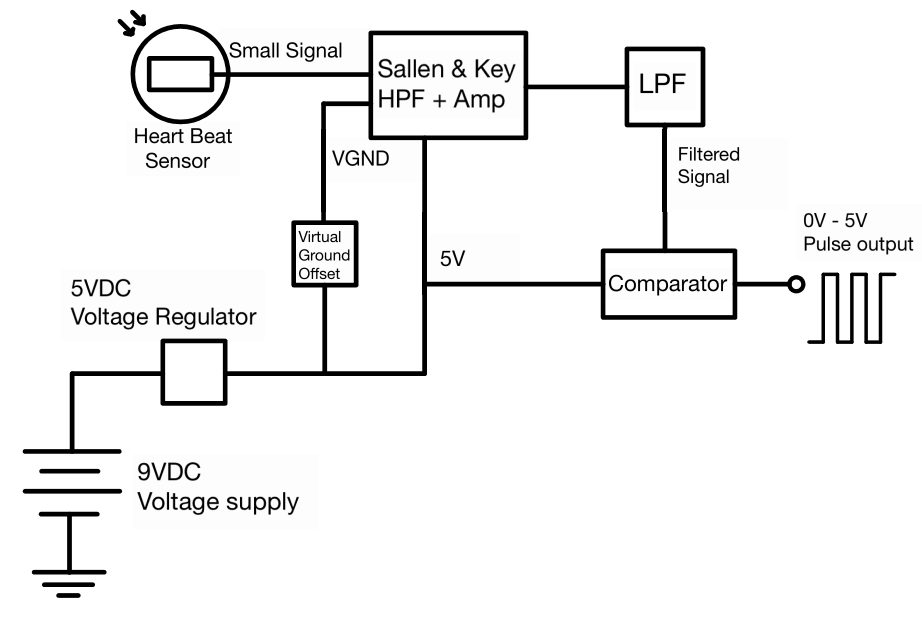
\includegraphics[width = 0.8\linewidth]{Figures/SysDiagram.png}
    \caption[System Block Diagram]{System diagram}
    \label{fig:system_diagram}
\end{figure}

\vfill









